\section{Speed Acquisition Channel}\label{sec:speed-acquisition-channel}

	\subsection{CKP Signal Conditioning}\label{ssec:ckp-signal-conditioning-circuit}

		As mentioned in Section \ref{ssec:crankshaft-position-sensor}, a CKP sensor has a analog signal with variable amplitude. For this project the only important parameter to extract from the sensor output signal in order to obtain the wheel speed is its frequency (angular velocity). The most practical way to obtain this data is to use a tachometer interface circuit, for this project the LM2907 from \textit{Texas Instruments} \cite{lm2907-datasheet} will be used. LM2907 is a \textit{frequency-to-voltage} converter with a ground-referenced tachometer input with $\pm$28V maximum voltage, making it versatile for many different sensor models.
		
		\subsubsection{LM2907 Basic Tachometer Circuit}\label{sssec:lm2907-basic-tachometer-circuit}
			The conditioning circuit for this project was based on the \textit{Tachometer with Adjustable Zero Speed Voltage Output} on Figure \ref{fig:lm2907-minimum-component-tachometer} suggested by LM2907 datasheet \cite{lm2907-datasheet}.

			\begin{figure}[htbp]
				\centering
					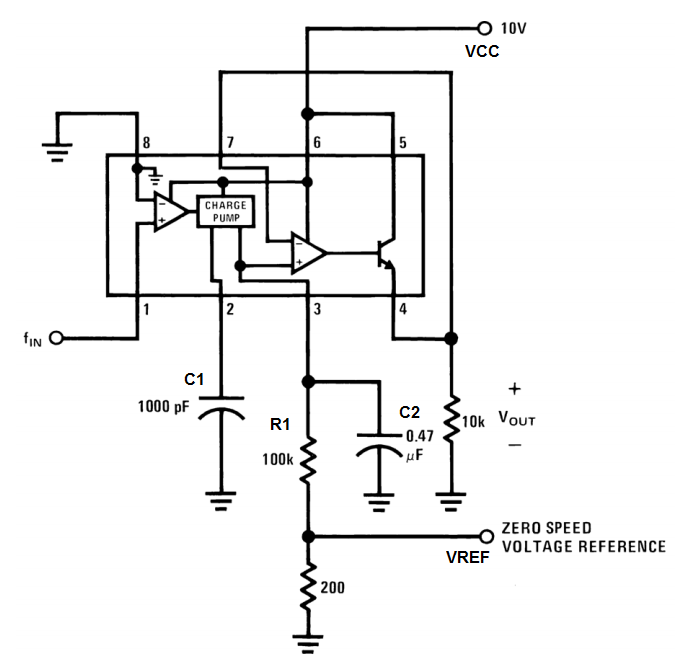
\includegraphics[scale=0.6]{figuras/fig-lm2907-minimum-component-tachometer.png}
				\caption{Tachometer with Adjustable Zero Speed Voltage Output, adapted from \cite{lm2907-minimum-component-tachometer}}
				\label{fig:lm2907-minimum-component-tachometer}
			\end{figure}

			According to the datasheet (\cite{lm2907-datasheet}), in order to configure the gain of the frequency-to-voltage converter, C1, R1 and C2 must configured in respect to the following design requirements.

			\begin{itemize}
				\item\textbf{\textit{C1:}} This capacitor is charged and discharged every cycle by a 180$\mu$A typical current source. C1 must not be sized lower than 500-pF due to its role in internal compensation.\label{itm:lm2907-c1}
				\item\textbf{\textit{R1:}} Higher of R1 values increase the output voltage for a given frequency, but too large will degrade the output’s linearity. Because the current pulses are a fixed magnitude of 180 $\mu$A  typical, R1 must be big enough to produce the maximum desired output voltage at maximum input frequency. At maximum input frequency the pulse train duty cycle is 100$\%$, therefore the average current is 180 $\mu$A and R1 = Vo(max) / 180 $\mu$A.\label{itm:lm2907-r1}
				\item\textbf{\textit{C2:}} This capacitor filters the ripple produced by the current pulses sourced by the charge pump. Large values reduce the output voltage ripple but increase the output’s response time to changes in input frequency.\label{itm:lm2907-c2}
			\end{itemize}

			The output voltage ($V_{O}$) can be calculated using Equation \ref{eqn:lm2907-output-voltage}, $V_{CC}$ is the supply voltage and $f_{IN}$ the input frequency.

			\begin{equation}\label{eqn:lm2907-output-voltage}
				V_{O}=V_{REF} + \left( V_{CC} \cdot f_{IN} \cdot C1 \cdot R1 \right)
			\end{equation}

			As said in Item \ref{itm:lm2907-c2}, C2 controls the voltage ripple on the output($V_{RIPPLE}$), this ripple is given by Equation \ref{eqn:lm2907-ripple}. According to the datasheet, $I_{2}$ has a typical value of 180uA.

			\begin{equation}\label{eqn:lm2907-ripple}
				V_{RIPPLE}=\frac{V_{CC}}{2} \cdot \frac{C1}{C2} \cdot \left( 1 - \frac{V_{CC} \cdot f_{IN} \cdot C1}{I_{2}} \right)
			\end{equation}

			Finally, the last thing to consider is the maximum attainable input frequency, determined by $V_{CC}$, C1 and $I_{2}$ (180uA) in Equation \ref{eqn:lm2907-max-freq}.

			\begin{equation}\label{eqn:lm2907-max-freq}
				f_{MAX} = \frac{I_{2}}{C1 \cdot V_{CC}}
			\end{equation}

		\subsubsection{LM2907 Designed Circuit}\label{sssec:lm2907-designed-circuit}

			The first parameter to be calculated is the maximum frequency, functional requirement from Item \ref{itm:func-req-5} in Section {sec:functionalRequirements} says the the system should be able to reach 200kph. Hence, to know the relation between frequency and speed on a wheel it's important to know the wheel's diameter. According to \cite{pneus-facil-todas-as-medidas-de-pneu}, the smallest commercial tyre size in terms of diameter in Brazil is the standard 165/70R13 which has a diameter (D) of 561.2mm and the one with the biggest diameter (D) is the standard 265/50R20 having 773mm. Using Equation \ref{eqn:diameter-to-length} to calculate the overall length of the wheel gives a aproximately length of 1.762m for the smaller tyre and a aproximately length of 2.428m for the bigger one.

			\begin{equation}\label{eqn:diameter-to-length}
				C = \pi \cdot D
			\end{equation}

			A speed of 200kph equals aproximately 55.5556m/s, using this value of speed divided by the calculated values of length, we have maximum frequencies of aproximately 31.52Hz (for the smaller tyre standard) and 22.88Hz (for the bigger tyre standard). Applying the greater value of frequency, a supply voltage of 5V (check Section \ref{ssec:the-choosen-mcu}) on Equation \ref{eqn:lm2907-max-freq} (remembering that $I_{2} equals$) gives a aproximately value of C1=1$\mu$F.
			\par
			Using this calculated value of C1 (1$\mu$F), with the maximum frequency (31.52Hz), the $V_{CC}$ value (5V), the desired offset voltage $V_{REF}$ (1V) and the maximum output voltage $V_{O}$ (5V) on Equation \ref{eqn:lm2907-output-voltage} gives a R1 value of 25.381k$\omega$, the closest commercial value is of 24k$\omega$, using this value gives a maximum output voltage in respect to the maximum input frequency of aproximately 4.78V.
			\par
			In Section \ref{ssec:the-choosen-mcu}, it is said that the choosen microcontroller's ADC has a resolution of 10-bit. A analog reference of 5V with 10-bit resolution gives a voltage resolution of 4.88mV. Hence, the calculated voltage ripple of the frequency-to-voltage converter must be less than the ADC resolution. Using values o $V_{RIPPLE}$, C1, R1, $f_{IN}$ and $V_{CC}$ in Equation \ref{eqn:lm2907-ripple} gives a C2 value of aproximately 63.75$\mu$F, the closest commercial value is 68$\mu$F.
			\par
			Figure \ref{fig:ckp-conditioning-circuit} shows the designed circuit for the speed acquisition channel.

			\begin{figure}[htbp]
				\centering
					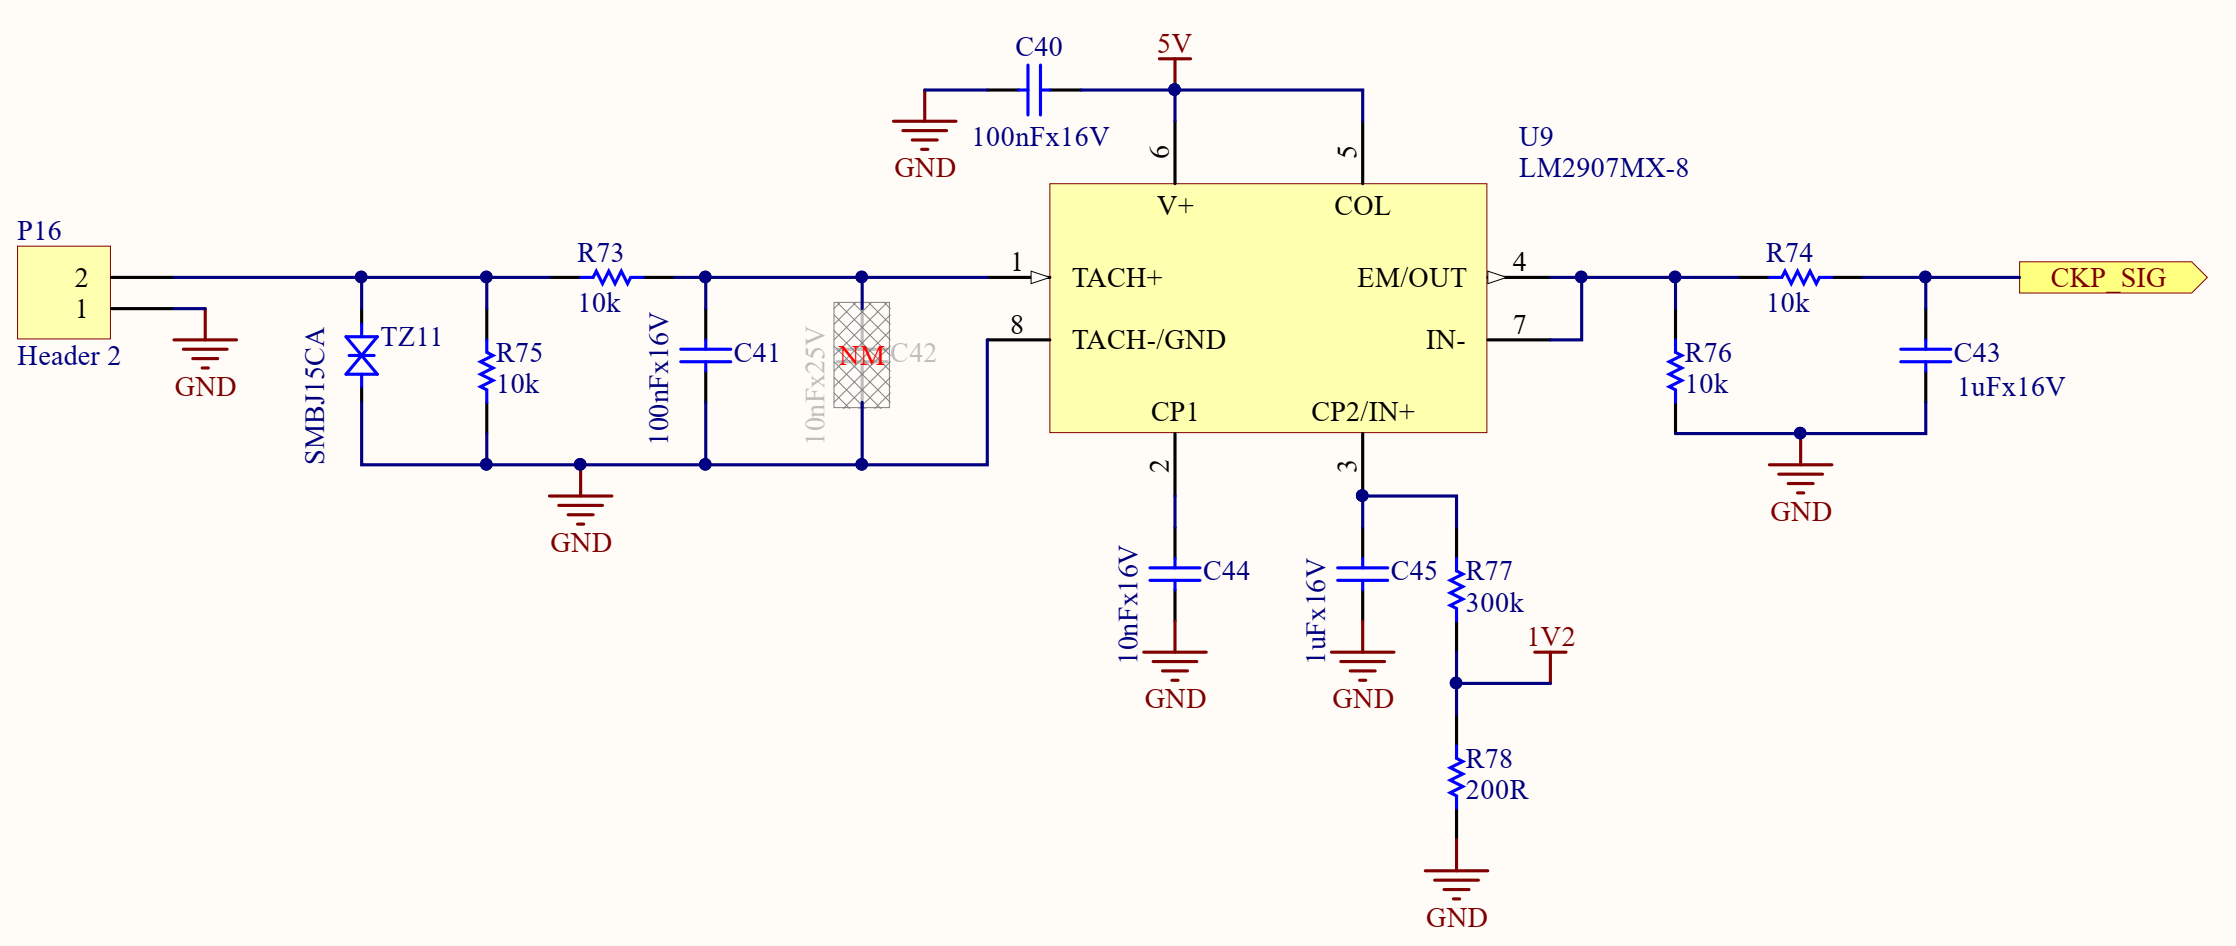
\includegraphics[scale=0.5]{figuras/fig-ckp-conditioning-circuit.png}
				\caption{Speed Acquisition Channel Circuit \cite{ckp-conditioning-circuit}}
				\label{fig:ckp-conditioning-circuit}
			\end{figure}

			In addition to the components from the circuit \textit{Tachometer with Adjustable Zero Speed Voltage Output} on Figure \ref{fig:lm2907-minimum-component-tachometer}, the following features have been added:

			\begin{itemize}
				\item\textit{\textbf{TVS Diode:}} In order to protect the the IC's input the SLD17-018 TVS diode from \textit{Littelfuse} was added. This diode has a maximum clamping voltage of 27.6V, the maximum input voltage is $\pm$28V, thus the TVS will protect the input from overvoltages.\label{itm:ckp-circuit-tvs}
				\item\textit{\textbf{LPF at the input:}} As the maximum frequency was determined to be 31.52Hz, it is possible to filter all the upper frequencies in order to avoid any noise to enter the circuit. R34 and C26 form a LPF with a cutoff frequency of aproximately 160Hz, this cutoff frequency was choosen because at 31.52Hz (maximum input frequency), the attenuation is quite close to 0dB (-0.15dB) and shall not affect the input signal.\label{itm:ckp-circuit-lpf-input}
				\item\textit{\textbf{LPF at the output:}} R62 and C25 form a LPF to that is used to filter any external post-conversion noise, it has a aproximate frequency of 16Hz.\label{itm:ckp-circuit-lpf-output} 
			\end{itemize}


	\subsection{CKP Sensor Detection}\label{ssec:ckp-sensor-detection-circuit}

		The detection circuit consists basically of a filtered digital input, a extra cable from the CKP power supply line will need to be wired in order to detect when the board sensor is connected. Naturally, when this cable is disconnected this extra wire input will have zero volts.

		Figure \ref{fig:ckp-detection-circuit} shows the detection circuit for the CKP sensor.

			\begin{figure}[htbp]
				\centering
					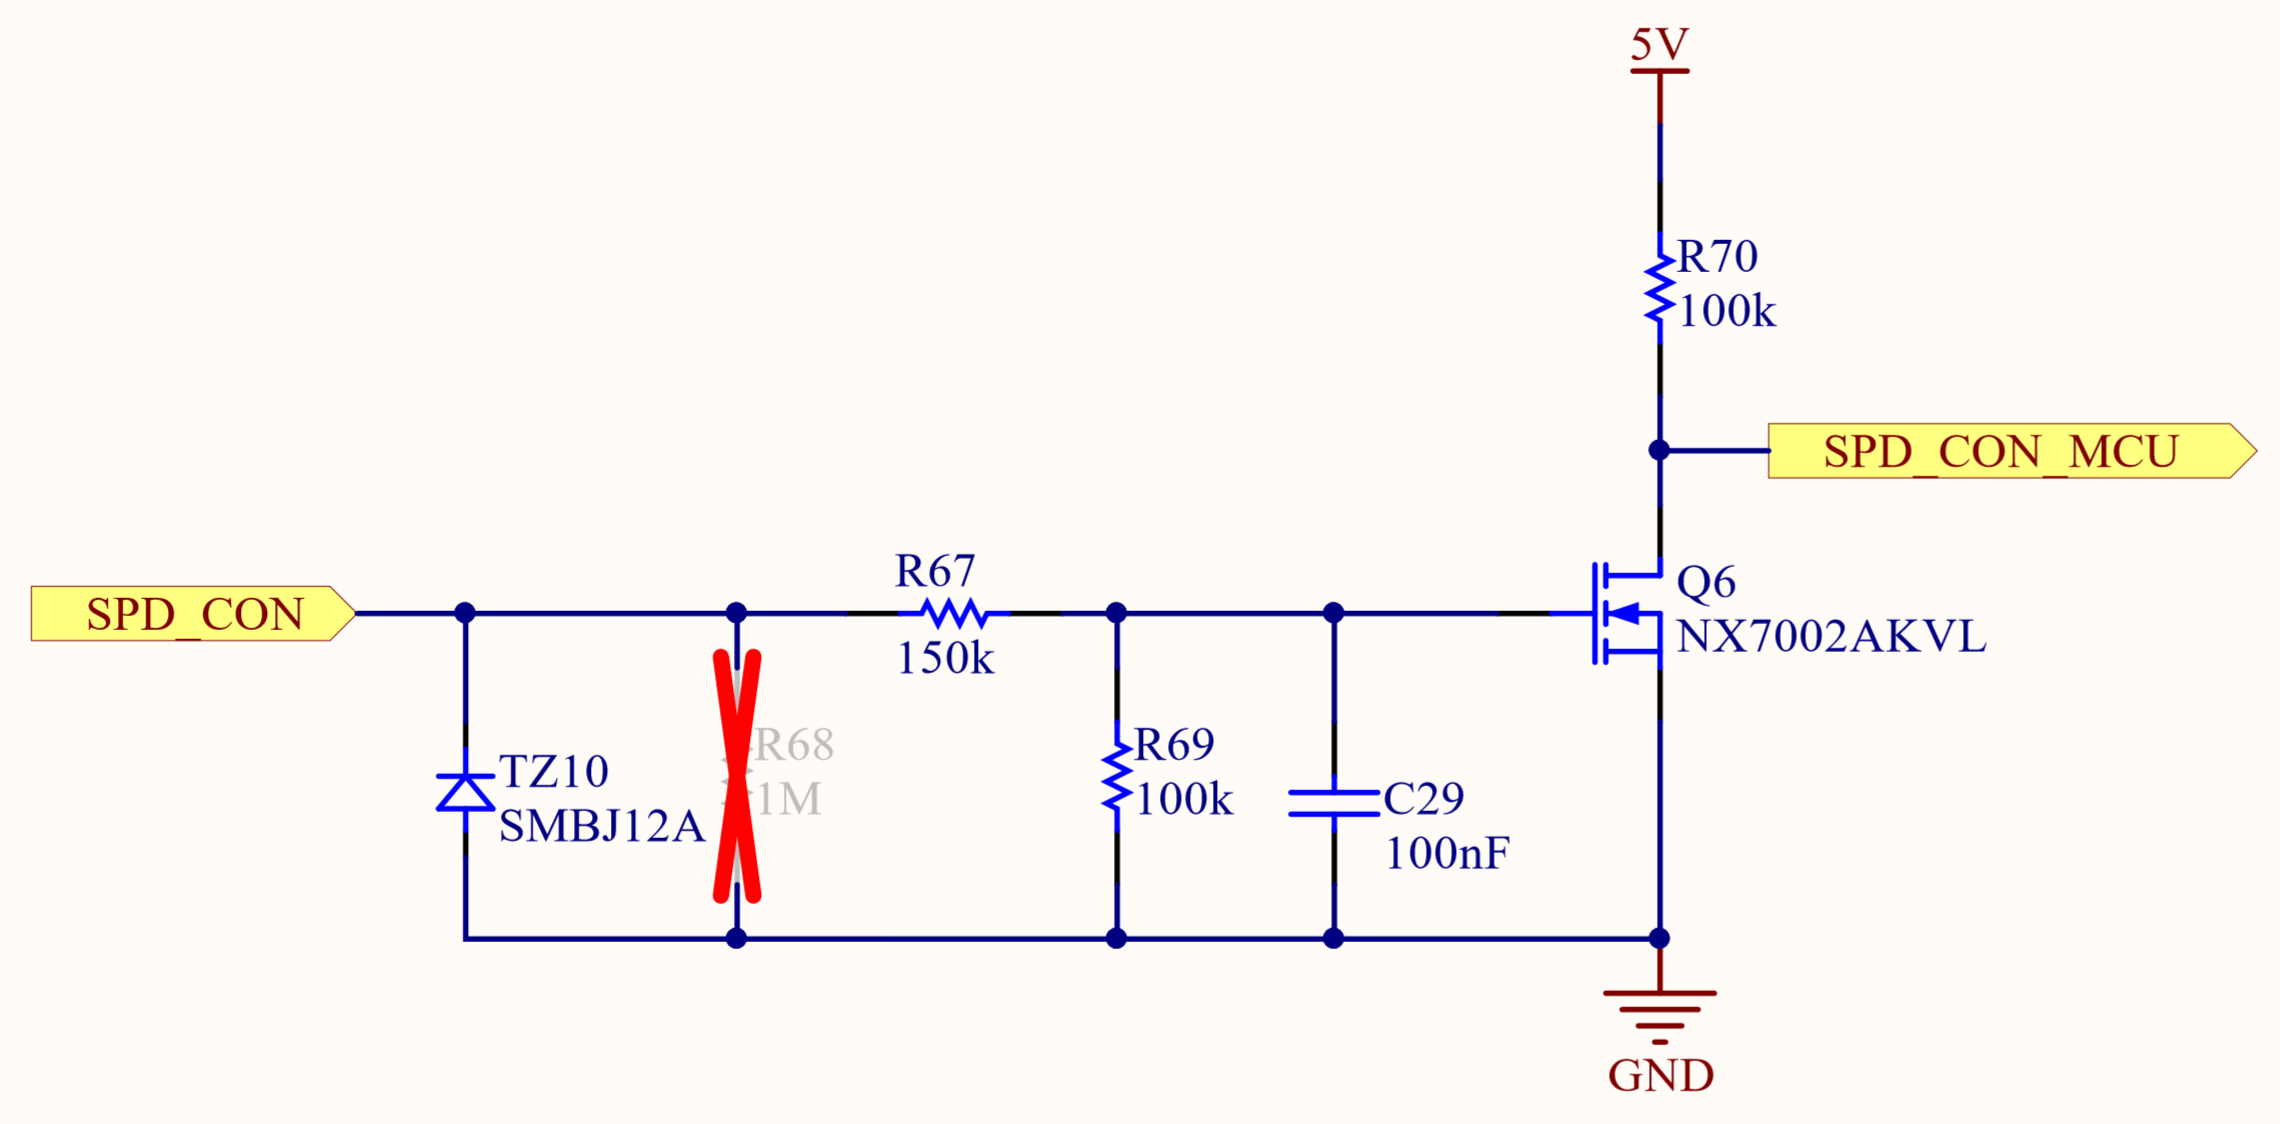
\includegraphics[scale=0.6]{figuras/fig-ckp-detection-circuit.png}
				\caption{Speed Sensor Detection Channel Circuit \cite{ckp-detection-circuit}}
				\label{fig:ckp-detection-circuit}
			\end{figure}

		TZ10 is TVS diode to protect the input from overvoltages. Resistors R67 and R69 form a voltage divider that will transform the 12V input signal to a 5V level signal. Resistor R67 and C29 form a LPF with cutoff frequency of 10.66Hz, this filter is used to attenuate unwanted noise from the input.